\begin{comment}
\section{Обзор существующих систем безопасности 
    уровня ядра ОС Linux и ОС Trusted BSD}

\bigskip
Сравним системы безопасности уровня ядра ОС Linux
(SELinux, AppArmor, GRSecurity) и Trusted BSD. 
Для сравнительного анализа были выбраны следующие 
критерии:

\bigskip
{\bfseries Реализованные модели безопасности.} 

    Существуют различные модели безопасности такие, 
    как Дискреционная(DAC), Мандатная(MAC), Принудительное 
    присвоение типов на основании определенной 
    политики(TE), Списки контроля доступа(ACL). 
    Данный критерий отражает реализованные 
    в рассматриваемой системе модели безопасности.  

\bigskip
{\bfseries Наличие возможности изменять матрицу доступа 
	во время исполнения.}
	
	Во многих из упомянутых выше моделях безопасности 
	контроль событий в системе осуществляется на основании 
	матрицы доступа. Матрица доступа это отображение
	декартова произведения множеств объектов и субъектов 
	системы на множество, элементами которого являются 
	наборы прав.
	Критерий отражает, есть ли возможность изменять
	матрицу доступа во время исполнения. 

\bigskip 
{\bfseries Возможность динамической смены контекстов
	приложения.}
	
	Для учета внутреннего состояния приложения в 
	процессе контроля за его поведением может быть
	использована динамическая смена контекста безопасности 
	 приложения. 
	Критерий описывает, существует ли в рассматриваемой 
	системе возможность менять права приложения в процессе
	исполнения. 

\bigskip
{\bfseries Классы вредоносных действий, предотвращаемых 
	системой безопасности.}
	
	Разные системы безопасности предотвращают различные 
	классы вредоносных действий. Некоторые системы 
	идут по пути предотвращения заранее известных 
	действий злоумышленника, другие позволяют минимизировать 
	нанесенный ущерб от успешной атаки. Из-за этого на практике 
	часто приходится комбинировать различные системы безопасности.    

\bigskip
\subsection{SELinux} 
SELinux~--- система безопасности 
уровня ядра Linux, основанная на 
подсистеме LSM. LSM позволяет 
создавать модули безопасности. Данные модули 
должны реализовывать 
определенную логику принятия решений о 
разрешении или запрещении различных 
взаимодействий между объектами и субъектами 
системы. 

Под объектами системы здесь 
понимаются файлы, объекты межпрограммного 
взаимодействия, объекты сетевого взаимодействия 
и прочие. Субъекты представляют собой 
пользовательские процессы, демоны, ядро и.т.д..

SElinux обеспечивает возможность 
комплексной защиты системы, ограничивая поведение 
приложений и пользователей в рамках политик 
безопасности. В первую очередь, SELinux 
направлена на борьбу с успешными атаками, 
в частности, с атаками нулевого дня, когда 
уязвимость уже известна злоумышленнику, 
но лекарства еще не было выпущено. В таких 
случаях уязвимость локализируется на уровне 
политики. Компания Tresys ведет подсчет 
конкретных случаев угроз безопасности, которые, 
в частности, могли быть предотвращены SELinux. 
В их числе: переполнение буфера в Samba (may 
2007), Apache DoS (jun 2007), Mambo exploit (jul 
2007), hplip Security flaw (oct 2007). 

Конфигурация политик является 
сложной задачей из-за необходимости
описывать профили для каждого приложения 
вручную на на специальном языке описания
политик. Добавление новых профилей может повлечь 
за собой необходимость в модификации уже имеющихся 
профилей, что может привести к появлению 
ошибок и росту накладных расходов на 
администрирование системы.  

Схема работы SELinux заключается в следующем.
Имеется политика, описывающая типы объектов
и субъектов в системе и матрицу доступа,
содержащую для каждого из субъектов его права
на операции с любым из типов объектов. Когда
любой из процессов производит системный вызов
для доступа к какому-либо объекту, подсистема
ядра SELinux вычисляет, имеет ли тип данного процесса
права на доступ к типу запрашиваемого объекта.
Если таких прав нет, запрашивающему процессу
будет отказано в доступе к объекту. В противном
случае, доступ к объекту будет предоставлен.
Схематично работа SELinux изображена на рисунке
\ref{fig:selinux}.

\subsubsection {Реализованные модели безопасности.} 

Принудительное присвоение типов (TE). 

Основная идея принудительного присвоения
типов~--- явная разметка всех объектов 
в системе специальными структурами данных 
(метками безопасности), хранящими в себе информацию
об атрибутах объекта, используемую при принятии 
решений внутри логики политики. 
Для процессов и объектов используется 
один и тот же тип атрибутов. Поэтому достаточно 
одной матрицы для описания взаимодействий между 
разными типами, при этом объекты одного типа могут 
рассматриваться по-разному, если их их ассоциированные 
классы безопасности различны. Пользователи не 
привязаны к типам безопасности напрямую, вместо 
этого используется RBAC.

\bigskip
Ролевой контроль доступа (RBAC) 

Данный метод используется для определения 
множества ролей, которые могут 
быть назначены пользователям. SELinux расширяет 
модель RBAC до жесткой привязки пользовательских 
ролей к определенным доменам безопасности, роли 
могут быть организованы в виде иерархии приоритетов. 
Такая привязка ролей к доменам позволяет принимать 
большинство решений на основе конфигурации TE. 
Контекст безопасности, кроме всего прочего, включает 
в себя атрибут роли.

\bigskip
Многоуровневая система безопасности (MLS) 

SELinux предоставляет MLS для случаев, когда есть 
необходимость в традиционной многоуровневой системе 
безопасности. У объектов и субъектов могут быть 
различные уровни и категории. 
Как правило, используется лишь один уровень. 


\subsubsection{Наличие возможности изменять матрицу доступа 
	во время исполнения} 

SELinux Предоставляет возможность перезагружать 
	политику во время работы системы. 

\subsubsection{Возможность динамической смены контекстов
приложения} 
 
SELinux предоставляет разработчикам приложений 
инструментарий, позволяющий создавать более 
безопасные приложения. Этого можно достичь 
путем изменения текущих привилегий приложения 
во время его исполнения. 
Последнее реализуется путем изменения домена приложения. 
Приложение должно запросить у ядра ОС смену своего 
текущего домена на указанный. При этом возможность
такой смены доменов должна быть явно описана в 
политике безопасности. Далее данный метод будет
рассмотрен более подробно.  

\subsubsection{Классы вредоносных действий, предотвращаемых 
	системой безопасности} 

В отношении системы безопасности SELinux было бы неправильно 
говорить о предотвращении угроз. Кроме этого, система не 
оперирует классами угроз. Основной идеей SELinux является 
минимизация ущерба от успешных атак на приложение. Для 
этого накладываются жесткие рамки на поведение приложений. 
\end{comment}

\section{Обзор SELinux и SEAndroid}
\subsection{Общая терминология SELinux} 

На основе \cite{SEOF} введём некоторые общие понятия, используемые в
SELinux: 
\begin{description}
    \item{Тип} \hfill \\
        Определяет группу сущностей(процессов, файлов, сокетов и т.д.).
        Для процессов тип имеет специальное название — \emph{Домен}. На
        основе политики безопасности в SELinux определяется какие
        операции представители одного типа могут производить над
        представителям другого.  
    \item{Объект}  \hfill \\
        Сущность, через которую информация проходит к субъекту. Это
        могут быть каталоги, файлы, поля, экраны, клавиатуры, память,
        магнитные накопители, принтеры или любые другие устройства
        хранения/перемещения данных. В сущности это контейнер данных или
        ресурс системы, доступ к объекту фактически означает доступ к
        данным.  
    \item{Cубъект}  \hfill \\
        Любая активная сущность, вызывающая перемещение информации между
        объектами, т.е.  пользователь, пользовательский обработчик,
        системный процесс и т.д.  
    \item{Атрибут}  \hfill \\
        Абстракция операции или группы операций, которые субъект может
        выполнить над объектом, например, чтение процессом файла.  
    \item{Политика безопасности}  \hfill \\
        Набор правил определяющих возможности доступа субъектов к
        объектам. Правила представляются в виде тройки \{тип субъекта, тип
        объекта, атрибут\}. С помощью политик SELinux в системе можно
        реализовывать доступ на основе подходов разных формальных
        моделей безопасности: Role-Based Access Control (RBAC), Type
        Enforcement (TE), Multi-Level Security (MLS). TE является
        наиболее популярной в последнее время.   
    \item{Контекст}  \hfill \\
        Элемент правила политики безопасности, определяющий тип
        сущности. В случае TE это понятие эквивалентно типу.
\end{description}

\subsection{Архитектура SELinux} 
\begin{figure}
\centering
\subfloat{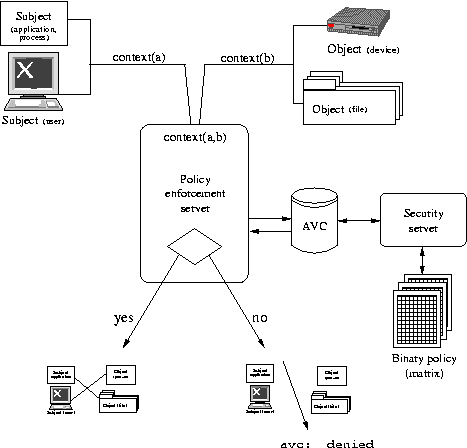
\includegraphics[width=110mm]{external/flask-arch.png}} 
\caption{Алгоритм принятия решений в SELinux}
\label{fig:selarch}
\end{figure}
Система SELinux состоит из следующих компонентов: сервер принятия
решений, кэш запросов и сервер политики.  SELinux также базируется на
Linux Security Modules (LSM, более подробно см. в \cite{LSM}), эта
система отвечает за отслеживание всех точек доступа к ресурсам
операционной системы через так называемые "хуки" в системных вызовах.
При попадании исполнения системного вызова на такой хук, LSM выполняет
проверку прав доступа приложения на возможность выполнения этого
системного вызова сначала через классическую систему Дискреционного
Контроля Доступа (DAC), а затем обращается к SELinux.  Общий алгоритм
работы SELinux в этом случае (проиллюстрирован на рисунке
\ref{fig:selarch}): 
\begin{itemize}
\item Процесс пытается выполнить операцию над объектом 
\item Сервер принятия решений получает уведомление от LSM о попытке
    провести операцию, получает контексты субъекта и объекта, а также
    атрибут операции от LSM и передаёт эту информацию серверу политики в
    виде запроса 
\item Сервер политики сначала проверяет в кэше наличие решения для
    такого запроса: разрешить или запретить операцию. Если решение
    найдено оно возвращается серверу принятия решения. Иначе ищется
    соответствующее правило в политике безопасности и на основе его
    принимается решение, помещается в кэш и опять же возвращается
    серверу принятия решений. Если правила не найдено то принимается
    решение запретить 
\item Сервер принятия решений на основе информации от сервера политики
    либо запрещает исполнение операции приложением (в этом случае,
    например, системный вызов аварийно завершается с кодом ошибки), либо
    позволяет продолжение выполнения операции 
\end{itemize}

\subsection{Политика SELinux} 

В качестве примера политики SELinux можно привести
фрагмент политики приложения OpenSSH.

\lstinputlisting[label=samplecode13,caption=Пример конфигурации модуля SELinux]{sourceCode/sepol.txt}
В данном фрагменте описывается тип процесса ssh\_t и
набор привилегий, предоставляемых данному типу:
\begin{itemize}
\item Set capability
\item Отлаживать процессы типа ssh\_t, исполнять свои сегменты
        кучи и стека
\item Использовать очереди сообщений
\item Отправлять и посылать сообщения
\item Использовать сокеты
\end{itemize}

Правила политики SELinux определяют неизменный набор привилегий для
процесса с соответствующим типом. Для изменения набора привилегий
процессу необходимо сменить тип, т.е. контекст. SELinux предоставляет
для этого несколько возможностей. Первая может быть определена в
политике через ключевое слово \emph{domain transition}. Такое правило
определяет для процесса возможность исполнять приложение другого типа
(совершать системный вызов execve). После того как новое приложение
начнёт исполнение, тип процесса будет изменён. Вторая возможность
предоставляется только для типов, у которых в политике задан атрибут
\emph{setattr}. Процессы такого типа могут совершать изменение своего типа на
любой другой, определённый в политике, с помощью библиотеки libselinux.
Как видно, в политиках SELinux нет возможности описать динамическое
изменение привилегий процесса для произвольного типа.

\subsection{SEAndroid}

Проект SEAndroid ставит перед собой цель добавить возможности мандатного
контроля доступа для улучшения безопасности Android-систем. Для этого
разработчики перенесли существующий фреймворк SELinux на платформу
Adroid, адаптировав его для использования в данной ОС. В частности, была
переделана стандартная политика SELinux, куда были внесены типы для
системных демонов, встречающихся в каждом устройстве на Android. Проект
базируется на открытой реализации Android проекте AOSP (Android Open
Source Project). На Android были портированы ряд патчей ядра, системные
утилиты для создания и редактирования политик, библиотека libselinux для
взаимодействия с SELinux из пользовательского пространства. 

Помимо прочего проект также ставит цель показать возможности SELinux и
MAC для ограничения системных сервисов, создания "песочниц", на Android.
На одной из презентаций разработчики показали, как SELinux мог быть
использован для предотвращения эксплуатации известной уязвимости
CVE-2011-1823, где злоумышленники использовали некорректную проверку
приходящих сообщений в демоне монтирования файловых систем vold для
исполнения произвольного кода с правами пользователя root.

\newpage

\begin{comment}
\subsubsection{Принципы работы}

Главными элементами системы безопасности 
являются субъект, объект и действия. В классы 
объектов входят классы файлов (blk\_file, chr\_
file, dir, fd,...\ ) ,  классы межпрограммного 
взаимодействия (ipc,msg,msgq,sem,shm), классы 
сетевого взаимодействия (key\_socket,netif,node,
packet\_socket,tcp\_socket), классы объектов 
(passwd), системные классы (capability, process,
Secutity, System). Под субъектами понимаются 
процессы, демоны, ядро и.т.д.. Действия, которые субъекты 
SELinux могут производить над объектами 
различны для различных классов объектов. 
Для классов файлов это, например, 
будут создание, исполнение, ссылки, чтение, запись, 
удаление. 

SELinux ассоциирует атрибуты безопасности 
с субъектами и объектами и основывает свои решения 
на этих атрибутах. Атрибутами являются: идентификатор 
пользователя, роль и тип. Идентификатор пользователя 
— пользовательская учетная запись, ассоциированная с 
субъектом или объектом. У каждого пользователя может 
быть несколько ролей, но в какой-то конкретный момент
времени ему может быть предписана только одна из них. 
Пользователь может менять роли командой newrole. Типы 
(для процессов~--- Домены) делят субъекты и объекты на родственные 
группы. Это~--— главный атрибут безопасности, используемый 
SELinux для принятия решений. 

Типы позволяют помещать 
процессы в "песочницы" и предотвращать повышение 
привилегий. К примеру, роль суперпользователя - 
sysadm\_r, его тип — sysadm\_t. Политика безопасности 
SELinux загружается системой из бинарного файла политики,
который, как правило, находится в /etc/selinux. 
Бинарная политика собирается при помощи make, исходные 
коды, как правило, находятся в /etc/selinux/\$(POLNAME)/src/policy.

Инструменты работы с SELinux могут быть разделены на 
три категории: специальные утилиты для настройки и 
использования SELinux, модифицированные версии стандартных 
команд и программ Linux, некоторые добавочные инструменты,
к примеру, для настройки и анализа политик. Среди основных 
команд можно выделить следующие: chcon – помечает файл или 
группу файлов указанным контекстом безопасности, checkpolicy
– позволяет выполнять множество действий, связанных с 
политиками, в том числе, компиляцию политики и ее загрузку 
в ядро; getenforce — позволяет узнать в каком режиме 
работает SELinux, newrole – позволяет пользователю 
перемещаться между ролями; run\_init — позволяет 
запускать, останавливать или контролировать сервис; 
setenforce позволяет менять режим работы системы; 
setfiles присваивает метки указанной директории и ее 
поддиректориям. Некоторые из измененных программ: cron, 
login, logrotate, pam, ssh. Некоторые инструменты: Apol 
– инструмент для анализа файла policy.conf; SeAudit – 
инструмент для анализа логов, имеющий графический интерфейс; 
SeCmds; SePCuT — инструмент для просмотра и редактирования 
файлов политик; SeUser — модификация пользовательских 
учетных записей. 
\end{comment}


